% Use the llncs.cls formatting
\documentclass{llncs}

% Set the packages for use within the document. The following 
% packages should be included.  Additional packages that do not
% conflict with these packages or change the llncs class formatting
% may be used.  Packages that do change the formatting are
% not allowed.
\usepackage{graphicx} % Used for displaying a sample figure. 
% If possible, figure files should be included in EPS format. 
% PDF format is also acceptable. JPEG  will work, but some of 
% them are downsampled resulting in fuzzy images.
\usepackage{pdfpages}
\usepackage{float}
\graphicspath{{./fig/}}
\usepackage{booktabs} % Better horizontal rules in tables
\usepackage{multirow} % Better combined rows in tables
\usepackage{amsmath}
\usepackage{array}
\usepackage{hyperref}

% The title of the papere remains a large amount of room for improvement.
% This is shite
\title{sEMG Gesture Recognition With a Simple Model of Attention}

% The complete list of authors with their affiliations
\author{%
David Josephs\inst{1} \and
Carson Drake\inst{1} \and
Che' Cobb\inst{1} \and
John Santerre\inst{1} %\and
%Jennifer Graves %triple verify graves still part of the team
}

% The Institutes and emails associated with each author. All students
% should use their MSDS affiliation or a generic SMU affiliation.
% Advisors should use their appropriate affiliation. Note that advisors
% are NOT referenced or otherwise denoted as advisors. Advisors
% are simply co-authors on the paper.
% Note that the emails for the MSDS affiliation, show how 
% to list emails that have the same organization portion.
\institute{%
Master of Science in Data Science, Southern Methodist University,
Dallas TX 75275 USA 
\email{\{josephsd, drakec, cobbc\}@smu.edu} %\and
%Springer Heidelberg, Tiergartenstr. 17, 69121 Heidelberg, Germany
%\email{lncs@springer.com} \\
%\url{http://www.springer.com/gp/computer-science/lncs} \and
%ABC Institute, Rupert-Karls-University Heidelberg, Heidelberg, Germany\\
%\email{\{abc,lncs\}@uni-heidelberg.de}
}
% Begin the document
\begin{document}

\maketitle              % typeset the title and author of the paper

% Reset the footnote counter
\setcounter{footnote}{0}

\begin{abstract}
This paper presents a novel method for fast classification of sEMG signals, using a simple model of attention. On a difficult, industry benchmark sEMG dataset, the proposed method yields excellent results, classifying 36 more gestures with about 20\% higher accuracy than the current standards in the field. These results have direct and immediate application in the fields of robotics, myoelctric control, and prosthetics.
\end{abstract}

\section{Introduction}

Electrophysiological studies of the nervous system are the core area of research in clinical neurophysiology, where scientists attempt to link electrical signals from the body to real world effects. These studies include measuring brain waves (electroencephalography), comparison of sensory stimuli to electrical signals in the central nervous system (evoked potential), and the measure of electrical signals in skeletal muscles (electromyography). \par
Electromyography is of particular interest to this paper. The nervous system uses electrical signals to communicate with the rest of the body. When a signal from the nervous system reaches a skeletal muscle, the myocytes (muscle cells) contract, causing a physical motion. By measuring these electrical signals in a supervised manner, we can develop a link between signal and physical action. This connection yields many powerful uses, ranging from quantifying physical veracity to diagnosing neurodegenerative diseases. An example of the latter can be found in Akhmadeev et al. \cite{graves}, where electromyographic (EMG) signals were used to classify Multiple Sclerosis patients from healthy control subjects with 82\% accuracy. \par
Deep learning can be used to further improve the power and utility of the EMG analysis. A deep neural network is, in essence, a composition of neurons (regressors) that learns a functional mapping between two sets of data. By learning a mapping between EMG signal and physical effect, we can develop more sensitive and accurate models of what connects the two. This also allows us to use less intrusive measurement devices in studies and in the real world. The applications of this range from clinical trials and prognostication of neuromuscular diseases to gesture prediction in "brain-controlled" prosthetic limbs. This study focuses on the latter application.
Current state of the art myoelectric prosthetic limbs  are capable of detecting and performing between 7 and 18 motions \cite{myohandpro} \cite{ottoblock}. While this represents a significant increase in the quality of life of an amputee, there remains a large amount of room for improvement. Most of the potential for improvement does not lie in the robotics themselves, which are fairly robust, but within the device which maps brain signal to motion of the hand. The aim of this paper is therefore to build a highly accurate gesture classifier using EMG signal, capable of classifying a broad range of gestures. \par
 Extending from this initial goal, there are certain metrics which must be met for the classifier to be deemed "useful". First, it must be fast. If there is a large degree of latency from thought to hand motion, the user will simply not use the device. Thus, it is important to determine the time window in which a prediction must be made. The absolute largest prediction latency for a model to be considered useful for myoelectric control lies between 250 and 300 milliseconds  \cite{300ms}, \cite{250ms}. For this study, the precedent set by \cite{primary} was followed, with a 260 millisecond prediction window.
Another key consideration for the classifier is generalizability. Within the field of myoelectric control and gesture recognition, there are two important types of generalizability, intra-subject and inter-subject \cite{ring_2018}. Intra subject generalizability indicates that the model is robust to personal elements, such as muscle fatigue. In contrast, inter-subject generalizability refers to the ability of the model to generalize to new people. This study focuses on intra-subject generalizability, as it is important that the device keep working for extended periods of time, while models can be fit to and personalized for amputees and non amputees alike \cite{amputeedb}. \par
In this paper, we propose a novel attentional architecture for sEMG recognition and myoelectric control. We demonstrate the model's validity on the 53-class NinaPro DB5 \cite{nina5}. We also compare different techniques  for dealing with the inherent class imbalance in sEMG, a synthetic data based approach (augmentation), an undersampling based approach, and a loss-based approach. All methods are evaluated on an intra-subject basis using the same holdout samples, yielding promising results.






%The absolute largest prediction latency for a model to be considered useful for myoelectric control lies between 250 and 300 milliseconds  \cite{300ms}, \cite{250ms}. Many recent papers claim excellent gesture prediction results, however they require time samples (windows) between 0.5 and 1.5 seconds long \cite{rnn_1000}, \cite{rnn_128}. In this paper, all windows are 260 milliseconds in length, following the precedent set by Allard et al. \cite{primary}. This leaves 40 milliseconds for any transformations done on the window, as well as the amount of time it takes for the model to make a prediction.



\section{Surface Electromyography}

Before discussing the mechanics of the proposed model, it is important to first discuss electromyography more closely. As mentioned in the Introduction, electromyography is the measure of electrical signals from the brain in the rest of the body. To be more specific, the body controls the forces in the muscles using electrical signals, via units called \emph{motor control units}, as seen in \autoref{fig:munit}. By measuring the amplitude and frequency of these signals, the strength or veracity of the motion and the type of motion can be determined. These signals are recorded in units of \emph{Motor Unit Action Potential}  (MUAP), either through internal electrodes or electrodes on the skin. This study is particularly focused on the measure of signals across the skin, or surface electromyography (sEMG). While sEMG is not quite as powerful as true EMG (e.g., the signals are weaker), it is far more practical and scalable, and far less disruptive, invasive, or sensitive to change. 
\begin{figure}[h]
\caption{%
A motor unit, consisting of: \emph{1} an Axon, \emph{2} a junction site, \emph{3} a Myocyte, and \emph{4} Myofibrils. The Axon sends electrical signal through the junction cite, causing the all of the myofibrils (and thus the entire myocyte) to contract.
}
\label{fig:munit}
\begin{center}
\fbox{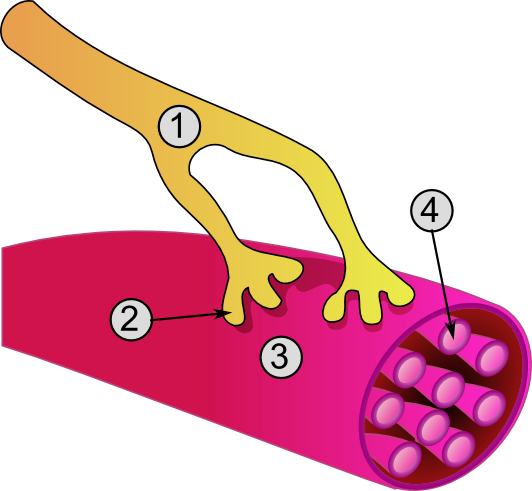
\includegraphics[height=5cm]{munit}}
\end{center}
\end{figure}
In this study, data are collected using two MYO armbands \cite{myo}, on the upper arm of the subject (just above the elbow), as seen in \autoref{fig:myoplace}. Intuitively, the idea is to collect the signal where the sensors are, and classify them with enough speed that it feels as if the hand were being moved on its own.
\begin{figure}[h]
\caption{%
The MYO armbands are placed just above the elbow.
}
\label{fig:myoplace}
\begin{center}
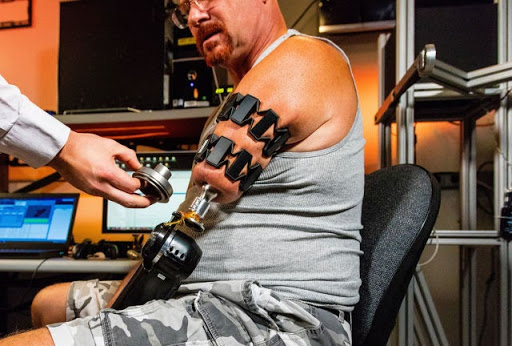
\includegraphics[scale=0.5]{myoplace}
\end{center}
\end{figure}


\subsection{The NinaPro Database}

The data in this study comes from the NinaPro Database, specifically database number 5 \cite{nina5}. Within this database, there are 52 unique motions measured, as well as rest, collected over 10 subjects. Each subject does each exercise 6 times, with 3 seconds of rest between each repetition. The signal from these are collected at the frequency of the MYO armband, 200 Hertz. 
\par This is one of the big challenges and benefits of the MYO armband. Low frequency sEMG is very sparse in information, and thus difficult to classify (especially relative to expensive HDsEMG sensors), however this also means that the MYO armband is cheap and accessible to the average consumer. The other benefit of MYOs cheapness and sparsity can be inferred from \autoref{fig:myoplace}. The cheap sensor constricts the arm and stays in place. Because the signals are weaker, slight shifts in the electrode do not have as much of an impact on the underlying signal (as the sensor is not incredibly sensitive). This means that the MYO armband is simpler and more robust for use by the general public.\par

The goal of this study is to develop an accurate mapping between MUAP in the upper arm and the motion of the hands.


\section{sEMG Classification}

In order to justify the need for deep sEMG classifiers, it is important to briefly discuss why shallow classifiers are inappropriate. Shallow classifiers (and really all of classical machine learning) relies on \emph{feature engineering}, or the creation of robust features which represent the data in a precise manner \cite{bddl}. This is very powerful, but it also comes with the assumption that the same fundamental process is generating all data points, that is the same feature set that works at time $a$ for person $x$ works at time $b$ for person $y$. However, in the case of surface electromyography, all brains and bodies are completely unique, which means that a classical, engineered feature set is neither robust between subjects or between repetitions (over time) \cite{dlot}. Therefore, we must turn to deep learning, to \emph{learn features from the data}, which are more robust over time and over subjects.

\subsection{Deep Learning}

Much of the previous work in sEMG classification (and time series classification in general \cite{dltsr}) with deep learning revolves around convolutional neural networks. In this subsection, notable and influential recent work will be highlighted. \cite{atz_cnn} very clearly demonstrated the power of convolutional neural networks with respect to sEMG classification, namely their flexibility and ease of use (due to feature learning vs feature engineering). This work is expanded in \cite{primary}, in which the authors use convolutional neural networks, wavelet transformations, and deep transfer learning to slightly improve on the results highlighted in \cite{atz_cnn}. \par
This study instead explores a new direction for both time series classification in general and for sEMG classification in particular: attention. In the last few years of language modeling, attentional models have proven more and more utilitarian, managing to solve problems of long term memory (which are commonplace in time series and language) while also managing to avoid the training and gradient issues of recurrent neural networks. Attention is a flexible, intuitive mechanism with lots of untapped application. In this study, the simple, feed-forward model of attention  described in \cite{raffel2015feedforward} is expanded upon. The attention mechanism is shown in \autoref{fig:okokt}. 


\begin{figure}[h]
\caption{%
A simple model of temporal attention.
}
\label{fig:okokt}
\begin{center}
\includegraphics[scale=0.75]{att}
\end{center}
\end{figure}

The mechanism works as follows: First time series data, an $(M,N)$ matrix (where $M$ represents timesteps and $N$ represents features or channels). This matrix is transposed into an $N$ by $M$ matrix. In this matrix, an observation at a single row represents all timesteps of that feature or channel. For example, row $x$ represents the time series produced by the feature $N = x$. This matrix is then fed in row by row to a standard, feedforward layer, using the softmax activation function. Thus, for each timestep of each feature, an importance (referred to as an "attention score") is calculated. Next, these are summed across time, producing a single number per feature, which represents the overall importance of the feature within that sample. As per \cite{raffel2015feedforward}, this simple mechanism, akin to a parametric time weighted average, actually successfully solves long term memory problems where order is not very important (or in this case, where memorization is to be avoided).


%\begin{figure}[h]
%\caption{%
%A motor unit, consisting of: \emph{1} an Axon, \emph{2} a junction site, \emph{3} a Myocyte, and \emph{4} Myofibrils. The Axon sends electrical signal through the junction cite, causing the all of the myofibrils (and thus the entire myocyte) to contract.
%}
%\begin{center}
%\label{fig:okok}
%\fbox{\includepdf[height=5cm]{fig/att}}
%\end{center}
%\end{figure}
%
%

\section{Data Processing}

Before any gestures can be predicted, the data must be prepared. There are two considerations for this. First, the preprocessing method must be fast and simple, as it needs to run with near zero latency on edge hardware (for example in a prosthetic hand). Second, the goal of using a deep neural network is to \emph{learn} robust features. Therefore, preprocessing methods must not profoundly alter the data, they must be simple methods which contain the maximum amount of available information. To start, the data (collected at 200 Hz), is sampled in time windows of 260 milliseconds (or 52 time steps), following the precedent set in \cite{primary}. One window of raw data can be seen in \autoref{fig:raw}.

\begin{figure}[h]
\caption{One window of sEMG data. The amplitude represents unitless motor activity potential, while the x axis represents the passage of time}
\label{fig:raw}
    \centering
    \def\svgwidth{0.7\columnwidth}
    \input{fig/raw.pdf_tex}
\end{figure}

This raw data represents what is collected by the two MYO armbands. Each armband collects 8-channel signal across the arm at 200 Hz. To remove any powerline interference, the armband collects the data with a notch filter which automatically removes the effects of large nearby electronics (such as power lines). The next step taken to make the signal more rich in information was to rectify (in layman's terms, take the absolute value of) the signal. In \cite{rectif}, it was shown that rectification significantly increased the availability of information pertaining to the  firing rate (temporal activity and pattern) of the motor units producing the signal. This means that rectification of the sEMG makes the information which allows for the learning of a pattern or feature which maps to a specific gesture more readily available.
\par After making the information denser, the next important preprocessing step is to make the information clearer. This is done in two ways. First, the packet of rectified signal is passed through a high pass Butterworth filter at 20 Hz. This removes any low frequency artifacts (aliases), which obscure the relevant signal. Finally, the data is passed through a moving average filter, which makes it more evident when the muscles are going through different periods of activity \cite{humancom}. The results of this preprocessing can be seen in \autoref{fig:proc}.
\begin{figure}[H]
\caption{One window of sEMG data. The amplitude represents unitless motor activity potential, while the x axis represents the passage of time. This data has been first rectified, then passed through a high pass filter, then passed through a 15-timestep moving average filter.}
\label{fig:proc}
    \centering
    \def\svgwidth{0.7\columnwidth}
    \input{fig/preprocessed.pdf_tex}
\end{figure}

\subsection{Data Augmentation}

One of the great challenges of deep learning, even with barely processed data, is its incredible capacity to overfit. In order to learn more robust mappings, without collecting a significantly larger amount of data, synthetic data must be generated, in order to prevent the deep learning algorithm from simply memorizing the training data. In this study, a novel data augmentation technique was employed, as seen in \autoref{fig:aug}. The methodology for the data augmentation is a simple random sample of a spectrum of different signal to noise ratios (SNR). A processed series is fed into the augmenter, and then random noise, at a given signal to noise ratio in magnitude is added. The signal to noise ratio for a realization is calculated at random as well, with linearly increasing likelihood as SNR increases. This allows the model to be trained for an extended period, without ever seeing the same observation twice.


\begin{figure}[H]
\caption{%
Data augmentation scheme, highlighted on a single channel of a single sample. Brighter realizations are more likely than dim ones.
}
\label{fig:aug}
\begin{center}
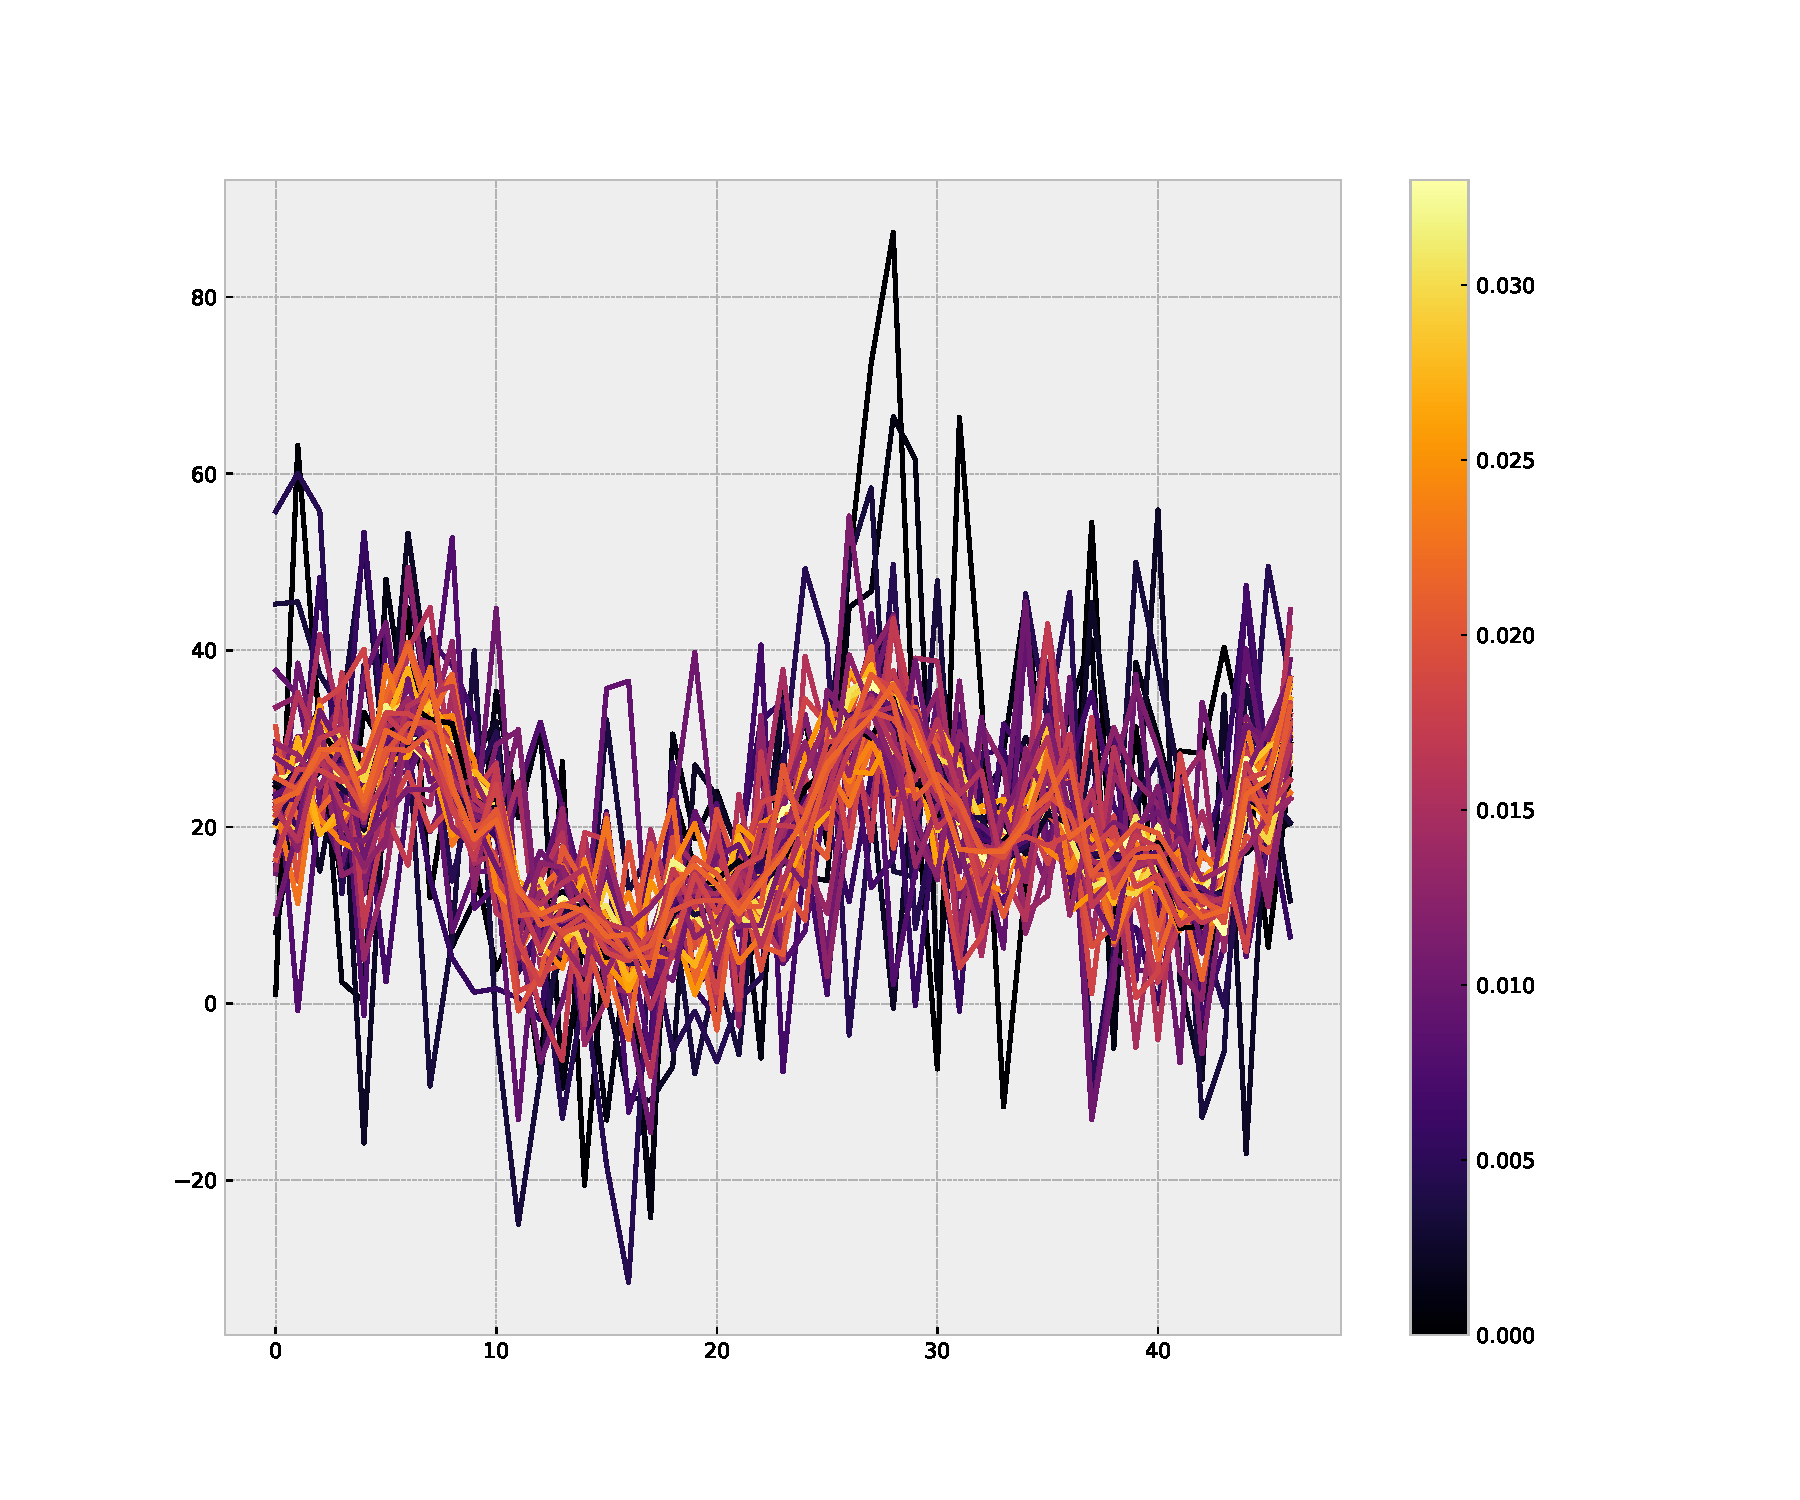
\includegraphics[scale=0.3]{augmentation}
\end{center}
\end{figure}

\section{Modeling}

The proposed model consists of three distinct phases: a convolutional preprocessor, an attention layer (as discussed in Section 3), and a classifier. 

\begin{figure}[H]
\caption{The proposed architecture. Red arrows represent dropout connections.}
\label{fig:mod}
\centering
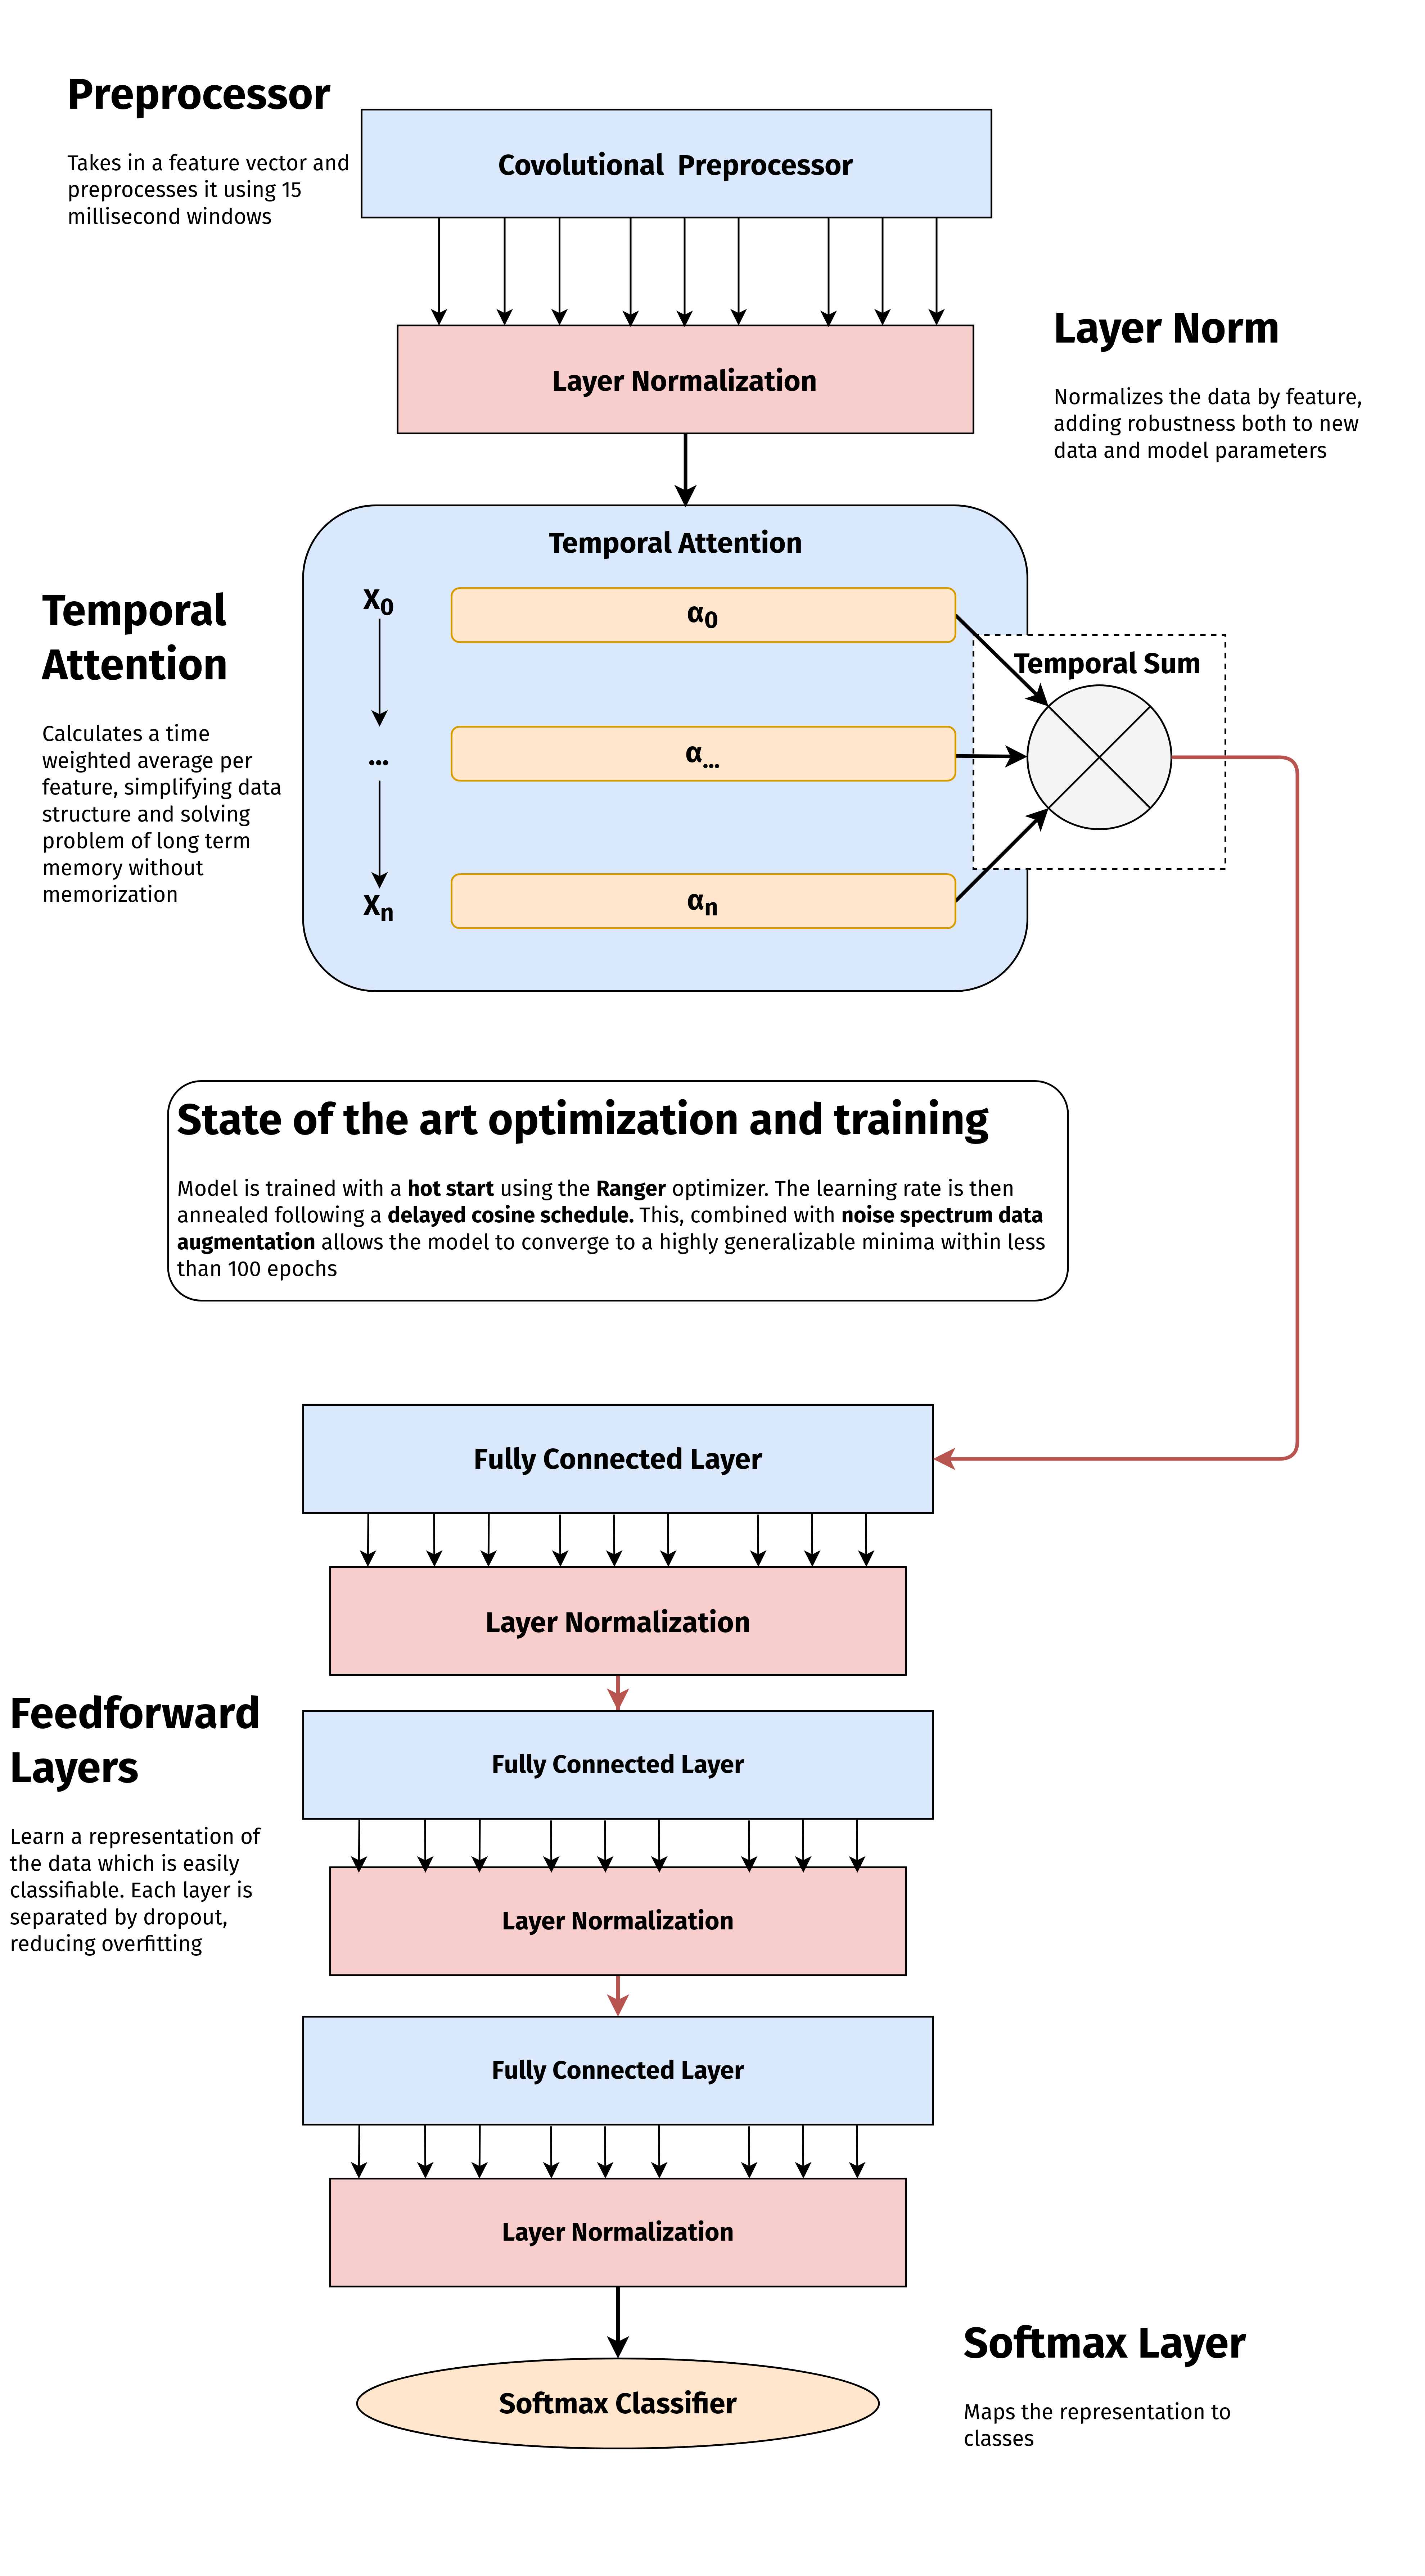
\includegraphics[width=\textwidth]{ntall}
\end{figure}

As seen in \autoref{fig:mod}, the first stage of the model consists of a single, 1-dimensional convolutional preprocessing layer. This  layer takes in the processed time series data, and filters them with a kernel size of three. That is, every three timesteps is filtered down into a single value (for each channel). This is done for each timestep, with 128 filters, resulting in a $(M, 128)$ matrix (where $M$ is the length of the time series). The output of this layer, and the output of all subsequent layers, are normalized across features (layer normalization) \cite{layernorm}. Layer normalization differs from batch normalization in that it normalizes across features, instead of across batches. Mathematically, consider a batch with dimensions $\bm{\left(\mathrm{samples }, \mathrm{timesteps }, \mathrm{features }\right)}$ (or, after attention, $\bm{\left(\mathrm{samples }, \mathrm{features }\right)}$). When batch normalization is applied, the weights are normalized using summary statistics across the \emph{samples}, while with layer normalization, the summary statistics used to normalize the weights are calculated across the \emph{features}.
\par
This matrix is then fed into the feed-forward attention mechanism described in \autoref{fig:okokt}, resulting in a feature vector of 128 values. These are fed into the classification network, which consists of a set of standard, feed-forward layers. The arhitecture of the classifier is based off of the architecture proposed  in \cite{dbn}, and was chosen due to its ability to effectively represent complex data. The output of this network is softmaxed in order to produce the final classifications. Each layer of the classification network is regularized using dropout.

\subsection{Training}

Several state of the art training techniques were employed in this model. First, instead of using the ReLU activation function, all layers use the "Mish" activation function \cite{mish}. The Mish activation function is slightly less regularized then ReLU, thus yielding results slightly faster (and avoiding the "dead neuron" problem). Instead of optimizing the network with Adam or SGD, the model was optimized using the Ranger optimizer. The Ranger optimizer consists of two components: Rectified Adam (RAdam) and Lookahead. The RAdam algorithm represents an improvement over the Adam optimizer in that it does not require a "warm up period", which Adam is notorious for needing. This allows the model to be trained to an optima much faster \cite{radam}. The Lookahead algorithm works in conjunction with a primary optimizer. The primary optimizer calculates weights as it normally does, and then the lookahead optimizer explores the loss landscape near the calculated weights. This allows for even faster convergence to an optima \cite{ranger2}. The combination of Lookahead and RAdam is the Ranger optimizer used in this paper \cite{ranger1}. Due to the very hot start of this combination (Mish and Ranger), the model learns very quickly. To further speed up training, the learning rate followed a delayed cosine annealing schedule. For the first 5 epochs, the model trains at a very high learning rate, and is subsequently annealed over the course of 50 epochs to a very low learning rate. This allows the model to quickly propel itself to a flat optima, and then work towards the bottom. This "hot start" methodology allows the model to quickly converge to a robust local minima \cite{break}.

A significant issue in sEMG classification is the large class imbalance present in the data. Most of the time, the hand is at rest. In the Nina 5 dataset, this means that there was over 30 times rest as any of the other 53 classes (and this also means that a non movable prosthetic hand would be about 60\% accurate). Three methods were tested to combat this imbalance. First, undersampling the majority class (rest), so that it would have the same likelihood of occurring in the training dataset as the other classes yielded decent results. A similar approach, augmenting all the minority classes to match the majority class, was tested, however the slight benefit over undersampling was far outweighed by the prohibitive training cost of this method. Finally, a loss-based method was tested, using focal loss \cite{focal}. Focal loss is calculated in almost exactly the same manner as categorical cross entropy, except it gives a lower importance to well aligned (easy to classify) samples, and raises the importance of difficult samples. This yielded by far the best results. 

\section{Results}

\section{Conclusions}

In this study, a novel method for classifying sEMG signals for myoelectric control was highlighted. It was shown that using a simple attention mechanism and state of the art training techniques, a model can be built to accurately classify a broad range of gestures, in a short period of time. This has immediate applications in the field of prosthetics, and can be expanded to other body parts with relatively little difficulty. \par
One general flaw of this study in general is the use of supervised learning at all. The presence of labels in human motion is rather unintuitive. In the future, research should be expanded into reinforcement learning and imitation learning, potentially combined with computer vision, in order to develop more robust models with an infinite range of gestures.



% text here

 \bibliographystyle{splncs04}
 \bibliography{samplebib}
%
%% End the document
\end{document}
